\section{Empirical Evaluation}
  
In this section we compare the solutions for traffic networks modeled as a QTM
before and after the introduction of a public transit network.
%
We consider both fixed control, i.e., a non-adaptive control plan, and optimal
adaptive control obtained by solving the
MILP~(\ref{eq:objFunc},~\ref{c:turnProbAndMaxFlow}--\ref{c:pd:holdTransit}).
%
The obtained solutions are simulated using the
LP~(\ref{eq:objFunc},~\ref{c:turnProbAndMaxFlow}--\ref{c:10}) and their total
travel time and observed delay distribution are used as comparison metrics.
%
Our hypothesis is that the optimal adaptive approach is able to mitigate the
impact of introducing a public transit w.r.t.\ both metrics.
%
In the remainder of this section, we present how we compute fixed control plans
using CTM, the traffic networks considered in the experiments, our methodology,
and the results.






\subsection{Networks}

\begin{figure}[t!]
\centering
%  trim={<left> <lower> <right> <upper>}
\subfigure[]{
\label{fig:net:arterial}
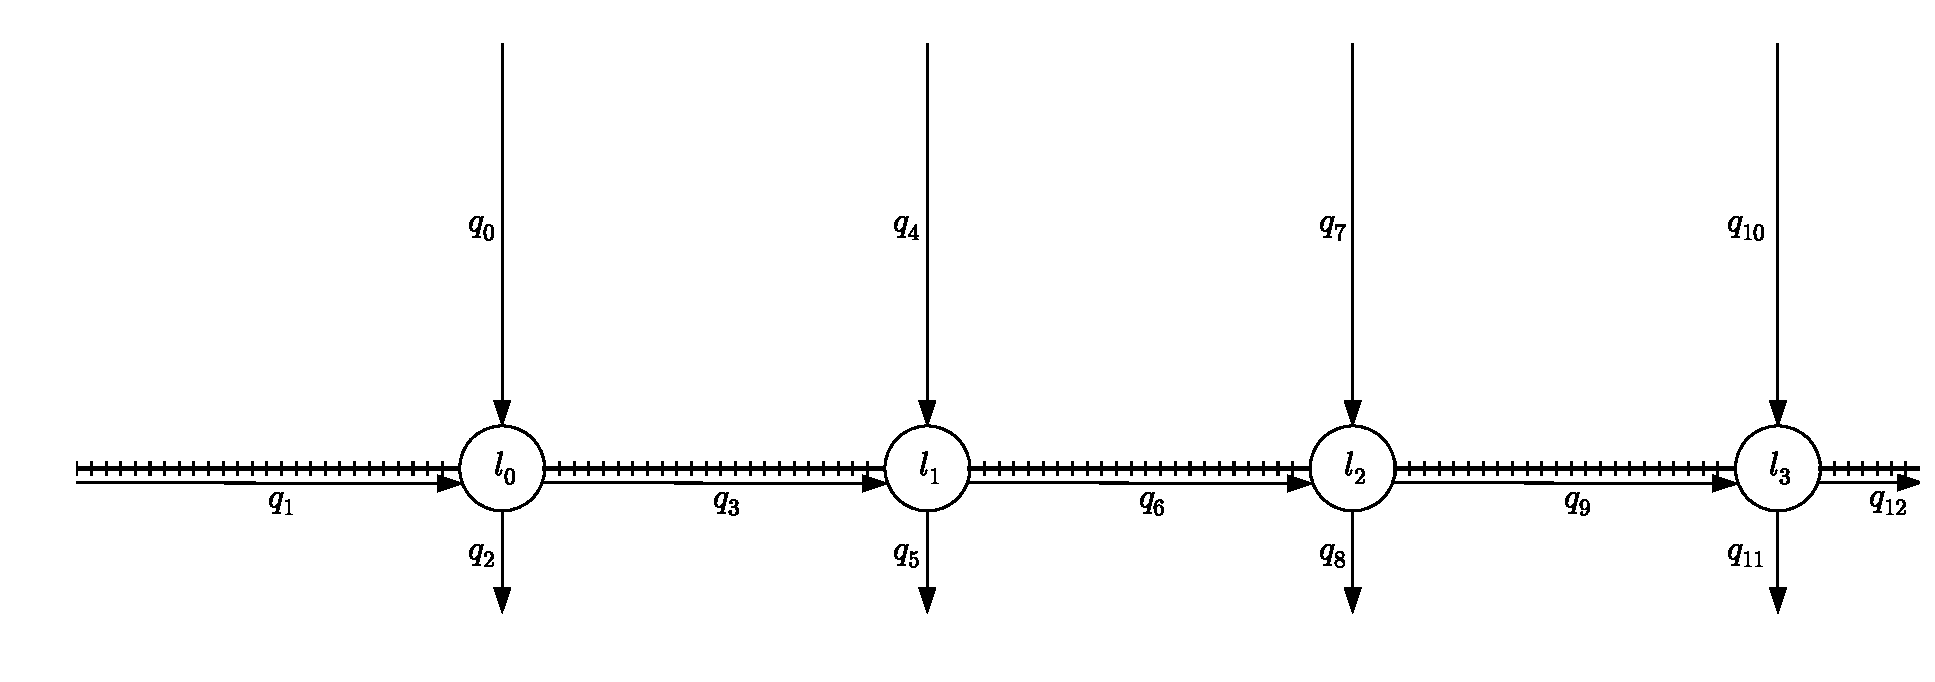
\includegraphics[width=0.47\textwidth]{network1.pdf}}
\subfigure[]{
\label{fig:net:grid}
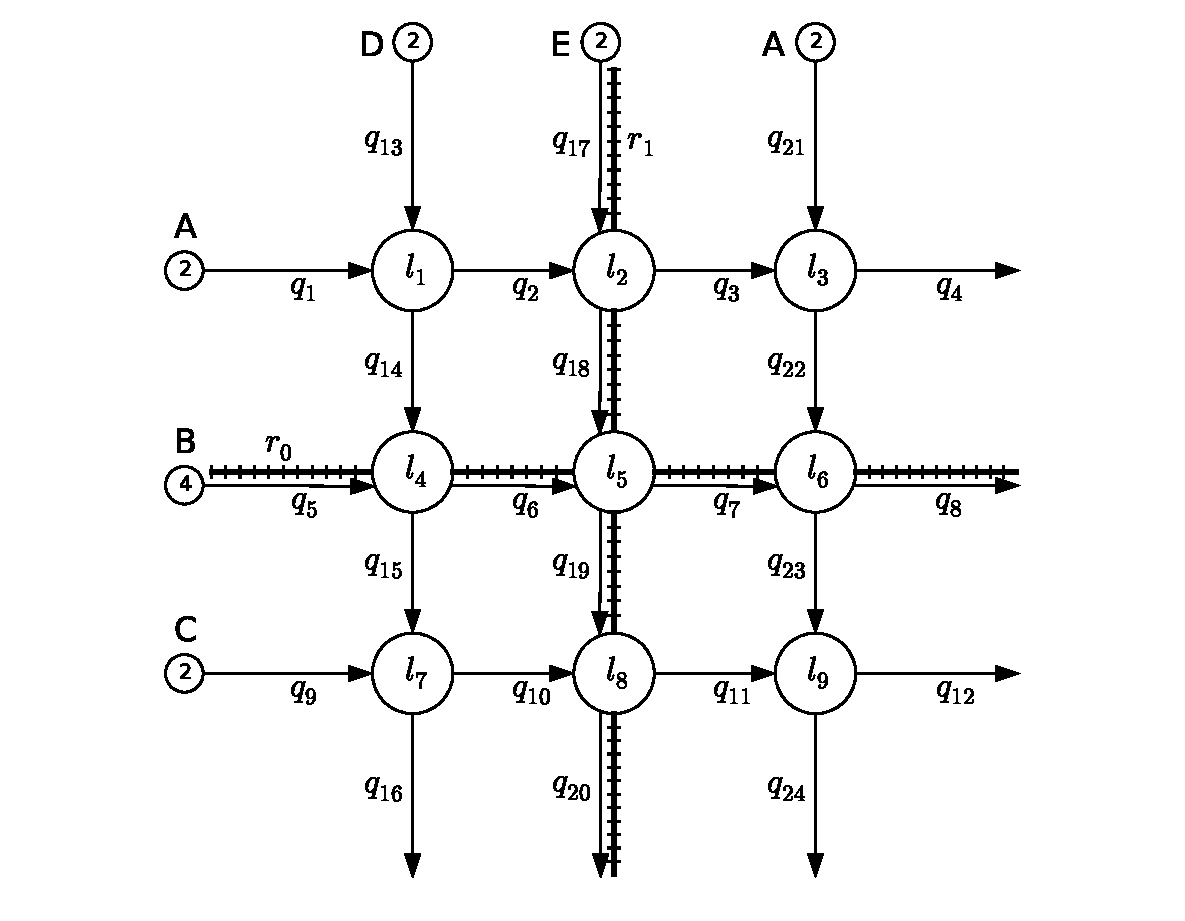
\includegraphics[width=0.40\textwidth]{network2.pdf}}
\caption{Networks used to evaluate the performance:
  (a) an arterial road with parallel light rail;
  (b) an urban grid with crisscrossing streets and light
  rail.
%
%(d) Demand profile of the queues marked as \qLowTraf,
  %\qHighTraf, and \qVarTraf for our experiments.
}
\label{fig:networks}
\end{figure}



We consider two networks of differing complexity: an arterial crossed by four
side streets (\cref{fig:net:arterial}) and a 3-by-3 grid (\cref{fig:net:grid}).
%
\authorHighlight{The queues receiving cars from outside of the network are
marked in \cref{fig:networks} and we refer to them as input queues.}\toIain{Make
sure to mark the new figure}
%
The maximum queue capacity~(\QMAX{i}) is 60 vehicles for non-input queues and
infinity for input queues to prevent interruption of the input demand due to
spill back from the stop line. 
%
The traversal time of each queue $i$~(\QDELAY{i}) is set at 30s,
\authorHighlight{except for the output queues on the grid where the traversal
time is 10s.}\toIain{Is this still true?}
%
For each street, flows are defined from the head of each queue $i$ into the tail
of the next queue $j$;
%
there is no turning traffic ($\FTURN{i}{j}=1$), and the maximum flow rate
between queues, \FMAX{i}{j}, is set at 0.5 vehicles/s.
%
All traffic lights have two phases, north-south and east-west, and for all
traffic light \tl and phase $k$, \PTMIN{\tl}{k} is 10s, \PTMAX{\tl}{k} is 30s,
\CTMIN{\tl} is 20s, and \CTMAX{\tl} is 60s.

\subsection{Fixed Phase Control Constraints}

We implement a fixed phase traffic light controller by replacing
$\pd[n]{\ell}{k} \le \PTMAX{\ell}{k}$  and \ref{c:minPhase}, with fixed duration
constraints employing the \textit{big-M} method to apply the constraints only
while the phase is inactive. The optimizer is free to choose a value for
$d^{fixed}_{\ell,k}$ within the bounds $\PTMIN{\ell}{k} \le d^{fixed}_{\ell,k}
\le \PTMAX{\ell}{k}$.

\begin{cAlign}
\pd{\ell}{k} &\le d^{fixed}_{\ell,k} + \PTMAX{\ell}{k} \p[n]{\ell}{k}
  \tagconstrain{c:pd:fixedUB}\\
%
\pd{\ell}{k} &\ge d^{fixed}_{\ell,k} - \PTMAX{\ell}{k} \p[n]{\ell}{k}
  \tagconstrain{c:pd:fixedLB}
\end{cAlign}
 
Constraints \ref{c:pd:fixedLB} and \ref{c:pd:fixedUB} are only applied for time
intervals $n$ where $\tn[n] > \CTMAX{\tl}$, to allow the controller to select an
optimized phase offset at the start of each plan.
%TODO talk about how the fixed phase times fit around transit crossings.


\subsection{Experimental Methodology}

Each network is evaluated at increasing demand levels up to the level where for
each queue $i$, $\inq{i}$ becomes saturated at $\QIN{i}{n}$.
%
\fnremark{FWT: we need to clarify that both approaches have access to the whole
``future'', i.e., perfect information about the incoming cars.}
%
For each demand level, traffic is injected into the network in bursts over 600s,
and \TMAX is set sufficiently high to allow all traffic to clear the network,
typically in the range 1000s to 1500s.\toIain{check horizons}
%
The pattern of the bursts and the value of $\QIN{i}{n}$ is marked on each input
queue in \cref{fig:networks}.\toIain{Add the new picture}
%
By clearing the network, we can easily measure the total travel time for all the
traffic as the area between the cumulative arrival and departure curves measured
at the boundaries of the network.
%
%TODO \fnremark{FWT: is this explanation of how to compute the total travel time
%still necessary?}
%
%\cref{tab:network_demand} presents the demand profile of each network.
%

We evaluate each network using the fixed control and the optimized control in
two scenarios: before the introduction of the introduction of the transit and
after its introduction. In both cases, we use \DT[] equal to 10s for all $n$.

For all experiments, we used Gurobi as the MILP solver running on a
heterogeneous cluster \authorHighlight{with 2.8GHz AMD Opteron~4184, 3.1GHz AMD
Opteron~4334 (12 cores each), and 2Ghz Intel Zeon E5405 (4 cores). We use 4
cores for each run of the solver.}\footnote{\authorHighlight{FWT: we can easily
cut this description in case we're 1 or 2 lines short.}}

We limit the MIP gap accuracy to 0.02\% and 0.1\% for the arterial and grid
networks, respectively.
%
Due to Gurobi's stochastic strategies, runtimes for the solver can vary,
and we do not set a time limit.
%
The optimal adaptive solution are typically found in real time, while fixed
control plans can take significantly longer; however, once the fixed control
solution is found, it can be deployed indefinitely.\toIain{Do you have the
cputimes by any chance in your log files so that we could say what is the
average?}




\subsection{Results}

\begin{figure*}[t!]
\centering
%  trim={<left> <lower> <right> <upper>}
\subfigure[]{
\label{subfig:travel_time_3}
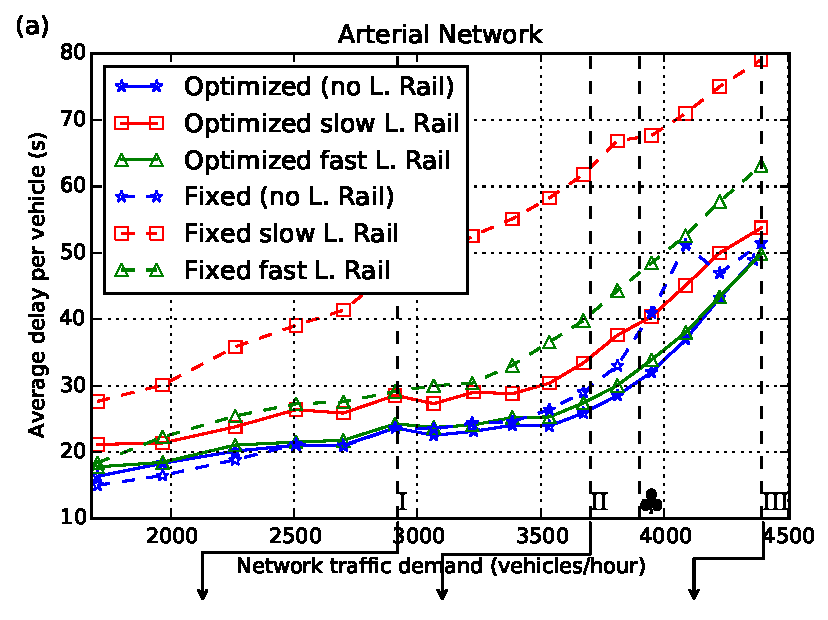
\includegraphics[keepaspectratio,height=0.3225\textwidth]{network1_delay.pdf}}
\subfigure[]{
\label{subfig:delay_3}
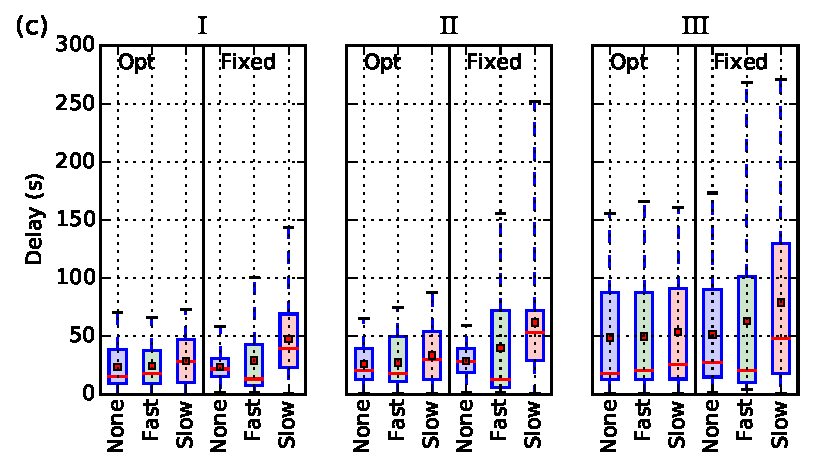
\includegraphics[keepaspectratio,height=0.3225\textwidth]{network1_boxplots.pdf}}
\caption{Increase in the total travel time w.r.t.~the optimal solution as a
function of \Nn (a,c,e) and distribution of the total delay of
each car for different values of \Nn (b,d,f).
%
For each row, the Roman numeral on top of the box plots corresponds to point the
travel time plot marked with the same numeral.
%
The mean of the total delay is presented as a red square in the box plots.
%
Plots in the $i$-th row correspond to the results for the $i$-th network in
\cref{fig:networks}.  Non-homogeneous (NH) achieves much better solutions
at smaller \Nn than Homogeneous (H).}
%control and achieves }
%smaller third quartile and maximum per-car delay for the same \Nn.}
\label{fig:results1}
\end{figure*}

\begin{figure*}[t!]
\centering
%  trim={<left> <lower> <right> <upper>}
\subfigure[]{
\label{subfig:travel_time_6}
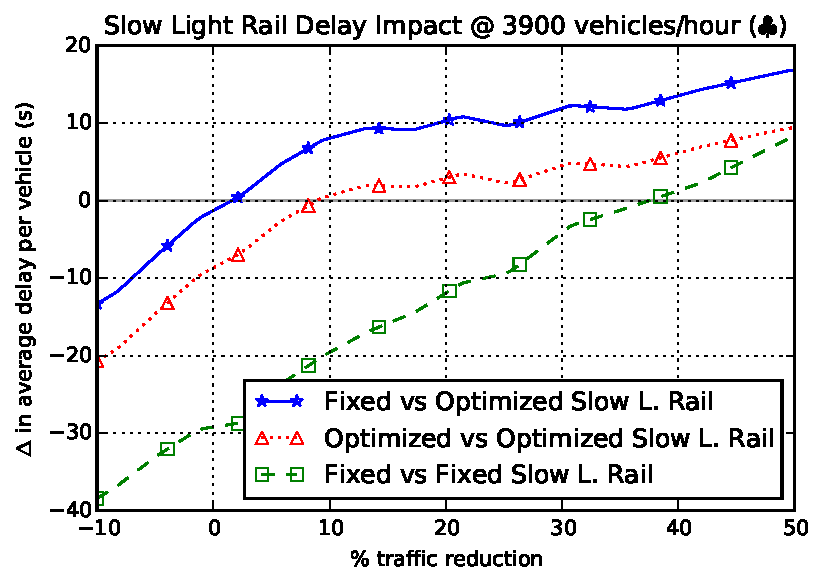
\includegraphics[keepaspectratio,height=0.3225\textwidth]{network1_t1_reduction.pdf}}
\subfigure[]{
\label{subfig:delay_6}
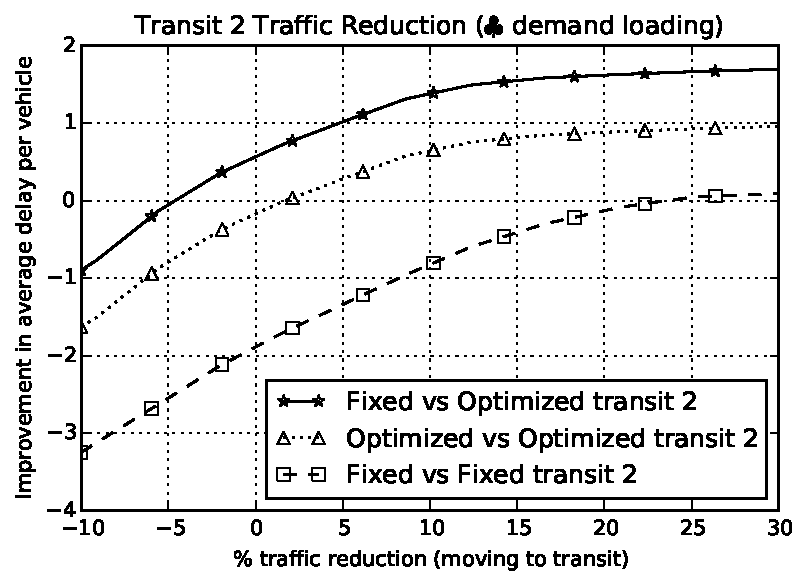
\includegraphics[keepaspectratio,height=0.3225\textwidth]{network1_t2_reduction.pdf}}
\caption{Increase in the total travel time w.r.t.~the optimal solution as a
function of \Nn (a,c,e) and distribution of the total delay of
each car for different values of \Nn (b,d,f).
%
For each row, the Roman numeral on top of the box plots corresponds to point the
travel time plot marked with the same numeral.
%
The mean of the total delay is presented as a red square in the box plots.
%
Plots in the $i$-th row correspond to the results for the $i$-th network in
\cref{fig:networks}.  Non-homogeneous (NH) achieves much better solutions
at smaller \Nn than Homogeneous (H).}
%control and achieves }
%smaller third quartile and maximum per-car delay for the same \Nn.}
\label{fig:results2}
\end{figure*}

\begin{figure*}[t!]
\centering
%  trim={<left> <lower> <right> <upper>}
\subfigure[]{
\label{subfig:travel_time_9}
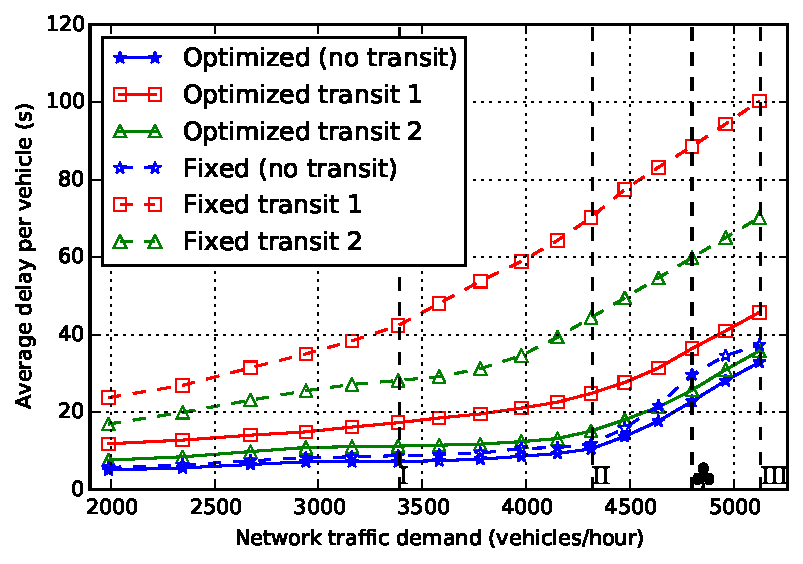
\includegraphics[keepaspectratio,height=0.3225\textwidth]{network2_delay.pdf}}
\subfigure[]{
\label{subfig:delay_9}
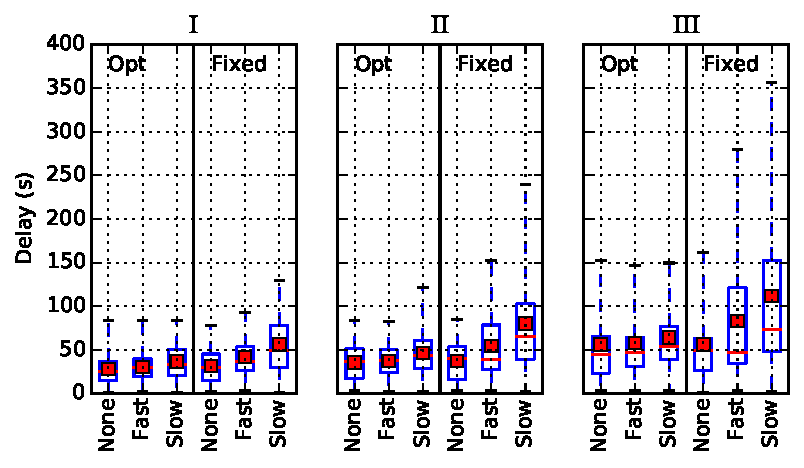
\includegraphics[keepaspectratio,height=0.3225\textwidth]{network2_boxplots.pdf}}
\caption{Increase in the total travel time w.r.t.~the optimal solution as a
function of \Nn (a,c,e) and distribution of the total delay of
each car for different values of \Nn (b,d,f).
%
For each row, the Roman numeral on top of the box plots corresponds to point the
travel time plot marked with the same numeral.
%
The mean of the total delay is presented as a red square in the box plots.
%
Plots in the $i$-th row correspond to the results for the $i$-th network in
\cref{fig:networks}.  Non-homogeneous (NH) achieves much better solutions
at smaller \Nn than Homogeneous (H).}
%control and achieves }
%smaller third quartile and maximum per-car delay for the same \Nn.}
\label{fig:results3}
\end{figure*}



\begin{figure*}[t!]
\centering
%  trim={<left> <lower> <right> <upper>}
\subfigure[]{
\label{subfig:travel_time_12}
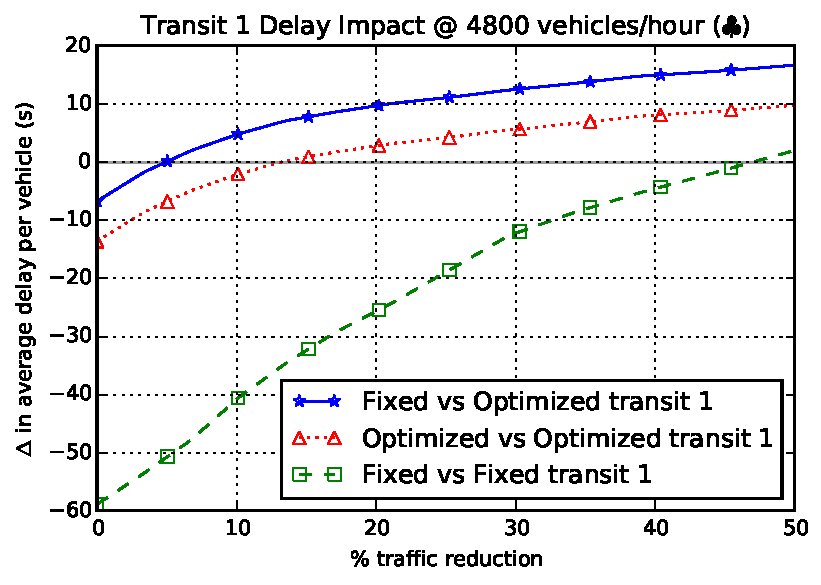
\includegraphics[keepaspectratio,height=0.3225\textwidth]{network2_t1_reduction.pdf}}
\subfigure[]{
\label{subfig:delay_12}
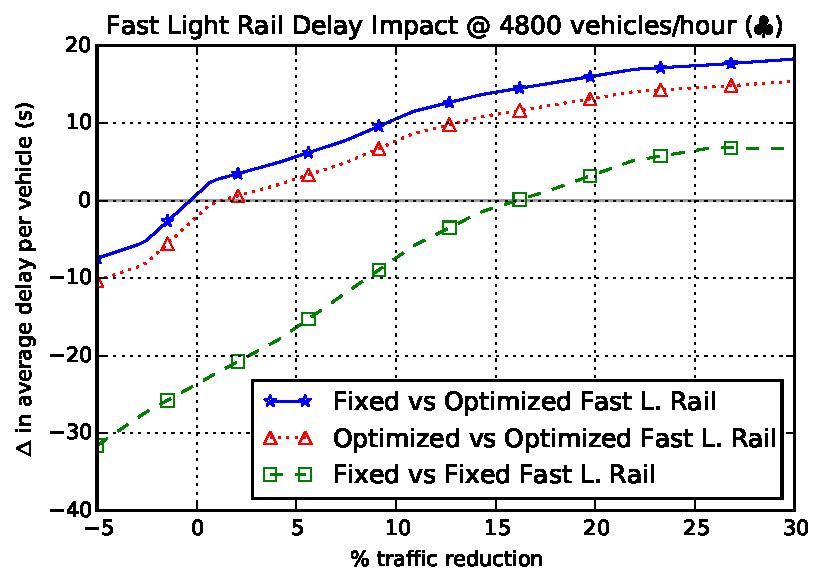
\includegraphics[keepaspectratio,height=0.3225\textwidth]{network2_t2_reduction.pdf}}
\caption{Increase in the total travel time w.r.t.~the optimal solution as a
function of \Nn (a,c,e) and distribution of the total delay of
each car for different values of \Nn (b,d,f).
%
For each row, the Roman numeral on top of the box plots corresponds to point the
travel time plot marked with the same numeral.
%
The mean of the total delay is presented as a red square in the box plots.
%
Plots in the $i$-th row correspond to the results for the $i$-th network in
\cref{fig:networks}.  Non-homogeneous (NH) achieves much better solutions
at smaller \Nn than Homogeneous (H).}
%control and achieves }
%smaller third quartile and maximum per-car delay for the same \Nn.}
\label{fig:results4}
\end{figure*}


%


%We compare the performance of non-homogeneous and homogeneous solutions in two
%ways: comparing the decrease in total travel time with increasing major frame
%time (greater look ahead), and analysing the distribution of delay in each
%queue of the network.
%
\cref{subfig:travel_time_3,subfig:travel_time_6,subfig:travel_time_9} show, for
each network, the increase in the total travel time w.r.t.~the optimal solution
as a function of \Nn.
%
As we hypothesized, the non-homogeneous discretization requires less time
intervals (i.e., smaller \Nn) to obtain a solution with the same total travel
time.
%
This is important because the size of the MILP, including the number of binary
variables, scales linearly with \Nn; therefore, the non-homogeneous approach can
scale up better than the homogeneous one (e.g., \cref{subfig:travel_time_9}).
%
Also, for homogeneous and non-homogeneous discretizations, finding the optimal
solution of major frames with large \Nn might require more time than our imposed
3000s time cutoff and, in this case, Gurobi returns a feasible control plan that
is far from optimal.
%
The effect in the total travel time of these poor solutions can be seen in
\cref{subfig:travel_time_9} for $\Nn > 120$.



The distribution of the total delay observed by each car while traversing the
network is shown in \cref{subfig:delay_3,subfig:delay_6,subfig:delay_9}.
%
Each group of box plots represents a different value of~\Nn: when the
non-homogeneous $\DT[]$ first converges; when the homogeneous~$\DT[]$ first
converges; and the optimum solution itself.
%
In all networks, the quality of the solution obtained using non-homogeneous
$\DT[]$ is better or equal than using homogeneous $\DT[]$ for fixed \Nn in both
the total travel time and \emph{fairness}, i.e., smaller third quartile and
maximum delay.

%\remark{FWT: In the paragraphs above, we need to address network 2 because it is
%the exception in both cases: in the end of \cref{subfig:travel_time_6},
%homogeneous is better, and the homogeneous delay in \cref{subfig:delay_6} is
%also better.}





To further illustrate the differences between homogeneous and non-homogeneous
discretizations, Figure (fig:cumu) shows the cumulative arrival and departure
curves and the how delay evolves over time for $q_1$ of network 2
(\cref{fig:net:grid}).
%
In Figure (subfig:cumu1), the comparison is done when non-homogeneous $\DT[]$
first converges (i.e., point I in \cref{subfig:travel_time_6}) and for this
value of \Nn, the major frame size in seconds of the non-homogeneous approach is
19.125s longer than the homogeneous one.
%
This allows the MILP solver to ``see'' 19s further in the future when using
non-homogeneous discretization and find a coordinated signal policy along the
avenue to dissipate the extra traffic that arrives at time 55s.
%
The shorter major frame of the homogeneous discretization does not allow the
solver to adapt this far in advance and its delay observed after 55s is much
larger than the non-homogeneous one.
%
Once the homogeneous $\DT[]$ has converged (Figure (cumu)), it is also
able to anticipate the increased demand and adapt well in advance and both
approaches generate solutions close to optimum (Figure (cumu)).
